\subsubsection{Mittlerer Atomabstand}
\begin{figure}[H]
\centering
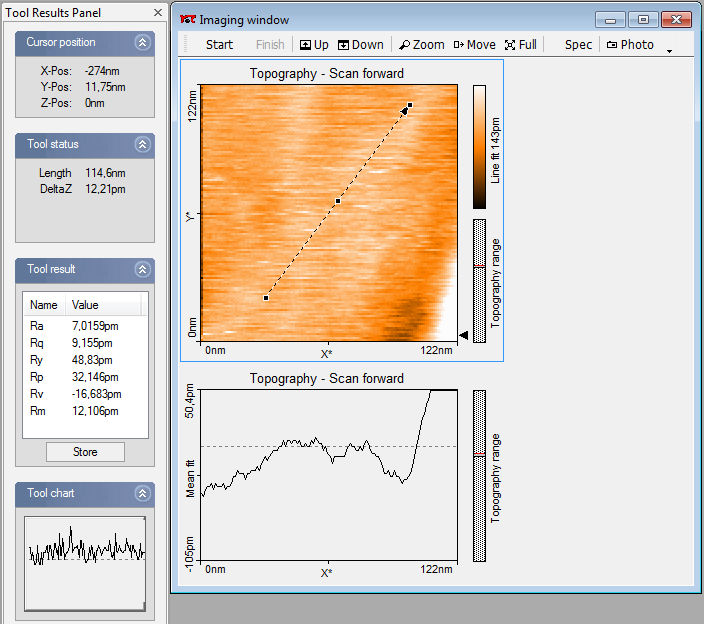
\includegraphics[scale = 0.75]{snipping_122_linienrauheit}
\caption{ Mittlere Linienrauheit von Graphit entlang der abgebildeten Linie \\ ($R_a = \SI{7,0159}{pm}$ und $R_q = \SI{9,1550}{pm}$) }
\label{fig:mittlere_Atomabstand}
\end{figure}